\chapter{Formal analogical proportions}
\label{CHAP:formal_analogical_proportions}

\initial{A}fter a first introduction of past works on analogical reasoning in
Chapter \ref{CHAP:computational_models_of_analogical_reasoning}, we will now
give all the necessary background on formal analogical proportions, the most
important concept of this document.

In Sections \ref{SEC:shortcut_from_aristotle_to_boolean_proportions} and
\ref{SEC:machine_learning_with_boolean_proportions}, we will guide the reader
through an insightful tutorial on the use of Boolean proportions and their
application to a small classification task. This will allow us to
introduce many of the key concepts used in the rest of our work, and to
illustrate their use with concrete examples. Please note that even if
these first two sections are quite informal, the concepts that they introduce
are all extremely important and it is crucial that they are well understood for
the rest of the document.  In Section \ref{SEC:formal_definitions_proportions},
will we provide finally provide the complete, formal definitions of analogical
proportion in algebraic settings.

Let us first start by diving into the realm of Boolean proportions.

\section{A shortcut from Aristotle to Boolean proportions}
\label{SEC:shortcut_from_aristotle_to_boolean_proportions}

In this first section, we will introduce the formal analogical proportions in a
Boolean setting, also mentioning the arithmetic proportion that is used when
dealing with real numbers. We will still make generic statements about
analogical proportions in general, regardless of the setting. We will use the
term \textit{analogical proportion} for such general statements.

\paragraph{The three axioms of an analogical proportion\\}

An \textbf{analogical proportion} is a statement of the form ``$a$ is to $b$ as
$c$ is to $d$'' involving analogical relations between the two pairs $(a,b)$ and
$(c,d)$, as well as between the two pairs $(a,c)$ and $(b,d)$.  There are numerous
examples of such statements, with which everybody will more or less agree, such
as  ``a calf is to a cow as a foal is to a mare'', or ``Paris is to France as
Berlin is to Germany''.

It has been agreed since Aristotle time that an analogical proportion $A$ is a
quaternary relation satisfying the three following axioms, for any $a, b, c, d$:

\begin{enumerate}
\item $A(a,b,a,b)$ always holds (Reflexivity)
\item $A(a,b,c,d) \implies A(c,d,a,b)$ (Symmetry)
\item $A(a,b,c,d) \implies A(a,c,b,d)$ (Central permutation)
\end{enumerate}

When there is no ambiguity over $A$ and its domain, the infix notation
$a:b::c:d$ is often used. Considering again our farm example, the symmetry
axiom states that if a calf $(a)$ is to a cow $(b)$ as a foal $(c$) is to a
mare $(d)$, then a foal $(c)$ is to a mare $(d)$ as a calf $(a)$ is to a cow
$(b)$, which seems perfectly sound. The central permutation axiom leads to the
natural consequence that a calf $(a)$ is to a foal $(c)$ as a cow $(b)$ is to a
mare $(d)$.

\paragraph{Equivalent analogical proportions\\}
Starting from the assertion $A(a, b, c, d)$ and by successive application of
the symmetry and central permutation axioms, we arrive to the following $8$
equivalent proportions:
\begin{align*}
       &A(a, b, c, d)\\
  \iff &A(c, d, a, b)\\
  \iff &A(c, a, d, b)\\
  \iff &A(d, b, c, a)\\
  \iff &A(d, c, b, a)\\
  \iff &A(b, a, d, c)\\
  \iff &A(b, d, a, c)\\
  \iff &A(a, c, b, d).
\end{align*}

If we applied one more time the central permutation axiom, we would end up with
our initial proportion $A(a,b,c,d)$: we say that these $8$ proportions
constitute an equivalent class. Note though that if $a, b, c, d$ are not all
distinct, this equivalent class contains less than $8$ proportions: for example
if $a = c$, then by the reflexivity axiom we must have that $b = d$, which
leads to the four equivalent proportions $A(a, b, c, d) \eqdef A(a, b, a, b)
\iff A(a, a, b, b) \iff A(b, b, a, a) \iff (b, a, b, a)$.

If we had started with the proportion $A(a,b,d,c)$, by successive applications
of the central permutation and symmetry axiom, we would have ended up again
with $8$ equivalents forms that are all different from those that are
\textit{generated} by $A(a, b, c, d)$. A third equivalent class is generated by
$A(a, c, d, b)$, and it is also composed of $8$ equivalent proportions that are
not present in the two other equivalent classes. In total, we end up with $24 =
3 \times 8$ distinct proportions, which correspond to the $24 = 4!$ possible
orderings of $a, b, c, d$.

\paragraph{The Boolean proportion\\}

There are various models of analogical proportions, depending on the target
domain. In section \ref{SEC:formal_definitions_proportions}, we will review
some definitions of analogical proportions in settings that are of interest for
us. But let us first focus on the \textbf{Boolean proportion}, i.e. proportions
dealing with Boolean numbers in $\mathbb{B} = \{0, 1\}$. The Boolean proportion
will indeed be one of the main object of study in this thesis.

The first axiom tells us that the proportion $a:b::a:b$ holds for any value of
$a$ and $b$ in $\mathbb{B}$. This means that the four following proportions are
valid:
\begin{itemize}
  \item $0 : 1 :: 0 :1$
  \item $1 : 0 :: 1 :0$
  \item $0 : 0 :: 0 :0$
  \item $1 : 1 :: 1 :1$
\end{itemize}

Using the central permutation axiom, we can derive two additional proportions:

\begin{itemize}
  \item $1 : 1 :: 0 : 0$
  \item $0 : 0 :: 1 : 1$
\end{itemize}

In a Boolean setting, there are exactly $2^4 = 16$ different valuations of $a,
b, c, d$. We have derived so far $6$ valuations (or \textbf{patterns}) that
lead to valid Boolean proportions, which are summed-up in Table
\ref{TAB:six_valid_patterns}. In Section
\ref{SEC:formal_definitions_proportions}, we will give a more formal definition
of Boolean proportions, indicating that the remaining $10$ patterns (also in
Table \ref{TAB:six_valid_patterns}) all lead to incorrect proportions.
\begin{table}[t]
  \centering
  \begin{tabular}[t]{ccccc}
    \toprule
    $a$ & $b$ & $c$ & $d$ &  $A(a, b, c, d)$\\
    \midrule
    0 & 0 & 0 & 0 &   \textbf{1}\\
    1 & 1 & 1 & 1 &   \textbf{1}\\
    0 & 0 & 1 & 1 &   \textbf{1}\\
    1 & 1 & 0 & 0 &   \textbf{1}\\
    0 & 1 & 0 & 1 &   \textbf{1}\\
    1 & 0 & 1 & 0 &   \textbf{1}\\
    \bottomrule
  \end{tabular}
  ~~~~
  \begin{tabular}[t]{ccccc}
    \toprule
    $a$ & $b$ & $c$ & $d$ &  $A(a, b, c, d)$\\
    \midrule
    0 & 0 & 0 & 1 &   \textbf{0}\\
    0 & 0 & 1 & 0 &   \textbf{0}\\
    0 & 1 & 0 & 0 &   \textbf{0}\\
    1 & 0 & 0 & 0 &   \textbf{0}\\
    1 & 1 & 1 & 0 &   \textbf{0}\\
    1 & 1 & 0 & 1 &   \textbf{0}\\
    1 & 0 & 1 & 1 &   \textbf{0}\\
    0 & 1 & 1 & 1 &   \textbf{0}\\
    0 & 1 & 1 & 0 &   \textbf{0}\\
    1 & 0 & 0 & 1 &   \textbf{0}\\
    \bottomrule
  \end{tabular}
  \caption{The six valid patterns of the Boolean proportion (left), and the ten
  invalid patterns (right).}
  \label{TAB:six_valid_patterns}
\end{table}

Table \ref{TAB:six_valid_patterns} provides us with valuable insights.  First,
it appears that the Boolean proportion can be defined in the following way:

\begin{definition}
  \label{DEF:boolean_proportion_informal}
  Four elements $a, b, c, d$ in $\mathbb{B}$ are in proportion if:
  $$
  \begin{cases}
    a = b \text{ and } c = d\\
    \text{or}\\
    a = c \text{ and } b = d.
  \end{cases}
  $$
\end{definition}

We also note from Table \ref{TAB:six_valid_patterns} that some sort of {\it
code independence axiom} is satisfied, which guarantees that $0$ and $1$ play
symmetric roles:

\begin{property}
  Let a, b, c, d in $\mathbb{B}$. Then
  $$a : b :: c : d \iff \neg a :  \neg b ::  \neg c :  \neg d,$$
  where $\neg x$ is the negation of $x$.
\end{property}

\paragraph{The arithmetic and geometric proportions\\}

If we consider that $\mathbb{B}$ is a subset of $\mathbb{R}$, (i.e. considering
that $a, b, c, d$ are now \textbf{real} numbers), it appears from Table
\ref{TAB:six_valid_patterns} that the Boolean proportion $a:b::c:d$ is true if
and only if $a - b = c - d$.

In fact, in general, a relation $a - b = c - d$ between four real numbers $a,
b, c, d$ is called an \textbf{arithmetic proportion}:
\begin{definition}
  Four elements $a, b, c, d$ in $\mathbb{R}$ are in \textbf{arithmetic
  proportion} if:
  $$a - b = c - d.$$
\end{definition}
We are here witnessing a close bond that links the Boolean proportion and the
arithmetic proportion: \textbf{when restricted to $\mathbb{B}$, the arithmetic
proportion and the Boolean proportion are equivalent}. The connections between
these two proportions will be more and more obvious as we go through this
document.

The arithmetic proportion, which states an equality of differences, is not the
only proportion that deals with numbers. The \textbf{geometric proportion} is
another instance of analogical proportion, which states an equality of ratios:
\begin{definition}
  Four elements $a, b, c, d$ in $\mathbb{R}$ are in \textbf{geometric
  proportion} if
  $$\frac{a}{b} = \frac{c}{d},$$
  or equivalently if
  $$a\times d = c\times b.$$
\end{definition}

Note that in $\mathbb{B}$ the geometric proportion offers a necessary condition
to define the Boolean proportion, but not a sufficient one: $a \times d =
b\times c$ is satisfied by all of the patterns in Table
\ref{TAB:six_valid_patterns}, but also for the pattern $0: 0: 0: 1$ which is
not a valid analogy. In that sense, the Boolean proportion is closer to the
arithmetic proportion than to the geometric proportion.

It should now be clear for the reader why analogical proportions are
effectively called \textit{proportions}: it's precisely because they generalize
the well-known numerical geometric proportion to more complex structures.
Actually, Aristotle stated the three aforementioned axioms on the basis of the
geometric proportion.

\paragraph{Analogical proportions over vectors\\}

Now, an analogical proportion in $\mathbb{B}$ is great, but what we are
interested in is a proportion in $\mathbb{B}^m$, to be able to deal with
Boolean vectors. A natural extension of the Boolean proportion to
$\mathbb{B}^m$ is to require that each of the $m$ dimensions make up valid
proportions in $\mathbb{B}$. This requirement can naturally be generalized to
any analogy over a set $X$:

\begin{definition}
  \label{DEF:analogy_for_vectors}
  Let $A$ be an analogy over a set $X$. We can define an analogy $A^m$ over
  $X^m$ in a component-wise fashion by:
  $$A^m(\mathbf{a}, \mathbf{b}, \mathbf{c}, \mathbf{d}) ~ \text{  if  } ~
  A(a_i, b_i, c_i, d_i) \text{ for all } i \in [1, m],$$
  where $\mathbf{a}, \mathbf{b}, \mathbf{c}, \mathbf{d}$ are vectors in $X^m$.
\end{definition}
\noindent
More often than not, $A^m$ will simply be denoted $A$ for the sake of brevity.
Let us also make a brief notation note: in the rest of these document, vectors
will be denoted by boldface letters and their components will be denoted by
regular letters. For example, a vector $\mathbf{x} \in X^m$ will be defined as
$\mathbf{x} = (x_1, x_2, \cdots, x_m)$.

So far we have seen a proportion in $\mathbb{B}$ and two proportions in
$\mathbb{R}$. Thanks to Definition \ref{DEF:analogy_for_vectors}, we now have
the definition of a proportion in $\mathbb{B}^m$, and two numerical proportions
in $\mathbb{R}^m$.  For example in $\mathbb{B}^2$, the four vectors $\mathbf{a}
= (0, 0),~ \mathbf{b} = (0, 1),~ \mathbf{c} = (1, 0)$ and $\mathbf{d} = (1, 1)$
are in proportion because the two component-wise proportions $a_1 : b_2 :: c_1
: d_1$ and $a_2 : b_2 :: c_2:d_2$ hold.

\paragraph{The Boolean and arithmetic proportions as parallelograms\\}

The interpretation of the geometric proportion in $\mathbb{R}^m$ can be opaque,
but that of the arithmetic proportion is very clear: four vectors $\mathbf{a},
\mathbf{b}, \mathbf{c}, \mathbf{d}$ of $\mathbb{R}^m$ are in arithmetic
proportion if $\mathbf{a} - \mathbf{b} = \mathbf{c} - \mathbf{d}$, i.e.
\textbf{if they are the four vertices of a parallelogram}, as illustrated in
Figure
\ref{FIG:arithmetic_proportion}.

\begin{figure}[!h]
\centering
  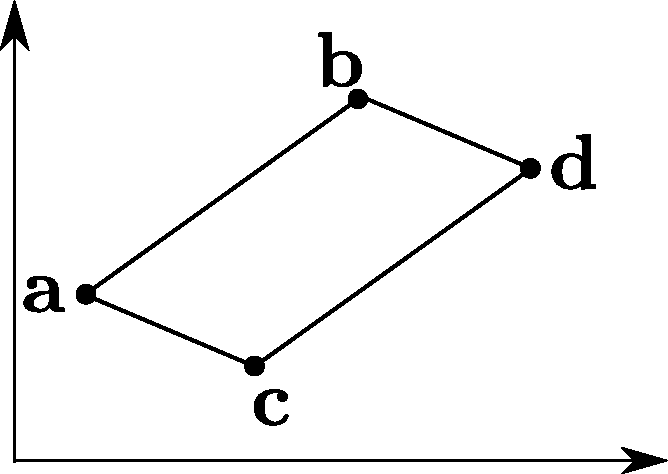
\includegraphics[width=2.5in]{figures/arithmetic_proportion.pdf}
  \caption{$\mathbf{a}, \mathbf{b}, \mathbf{c}, \mathbf{d}$
  are in arithmetic proportion iff they are the four vertices of a
  parallelogram.}
\label{FIG:arithmetic_proportion}
\end{figure}

Let us note that even if they did not explicitly mentioned the parallelogram
view of analogy, Rumelhart and Abrahamsen (Section
\ref{SEC:rumelhart_Abrahamsen}) clearly used the arithmetic proportion for
their model of analogical reasoning.

We have seen that in $\mathbb{B}$, and thus in $\mathbb{B}^m$, the Boolean
proportion and the arithmetic proportion are equivalent. This means that a
proportion in $\mathbb{B}^m$ can also be represented as a (potentially
\textit{flat}) parallelogram. By \textit{flat} parallelogram we mean that the
four vertices are not all distinct.  Figure \ref{FIG:proportions_in_B2}
illustrates the proportions that one can build in $\mathbb{B}^2$:
\begin{itemize}
  \item The proportion $\mathbf{a}: \mathbf{b} :: \mathbf{c} : \mathbf{d}$ and
    its 7 other equivalent forms, making up the parallelogram
    $\mathbf{a}\mathbf{b}\mathbf{c}\mathbf{d}$.
  \item The proportions that we can build using any pair of vertices, for
    example $\mathbf{a} : \mathbf{d} :: \mathbf{a} : \mathbf{d}$. Each of these
    proportions has $3$ other equivalent forms: in our case $\mathbf{a} :
    \mathbf{a} :: \mathbf{d} : \mathbf{d}$, $\mathbf{d} : \mathbf{a} ::
    \mathbf{d} : \mathbf{a}$ and $\mathbf{d} : \mathbf{d} :: \mathbf{a} :
    \mathbf{a}$. As there are $\binom{4}{2} = 6$ pairs of vertices in
    $\mathbb{B}^2$, there are exactly $6 \times 4$ proportions of this kind,
    all of which are flat\footnote{\textit{flat} proportion are those that make
    up flat parallelograms. This naming convention is actually fortunate,
    because these proportions are in practice absolutely useless, as it will
    soon become clear.}.
  \item The $4$ proportions involving each vertex independently, for example
    $\mathbf{b}:\mathbf{b}::\mathbf{b}:\mathbf{b}$. These proportions are also
    flat, naturally.
\end{itemize}

\begin{figure}[!h]
\centering
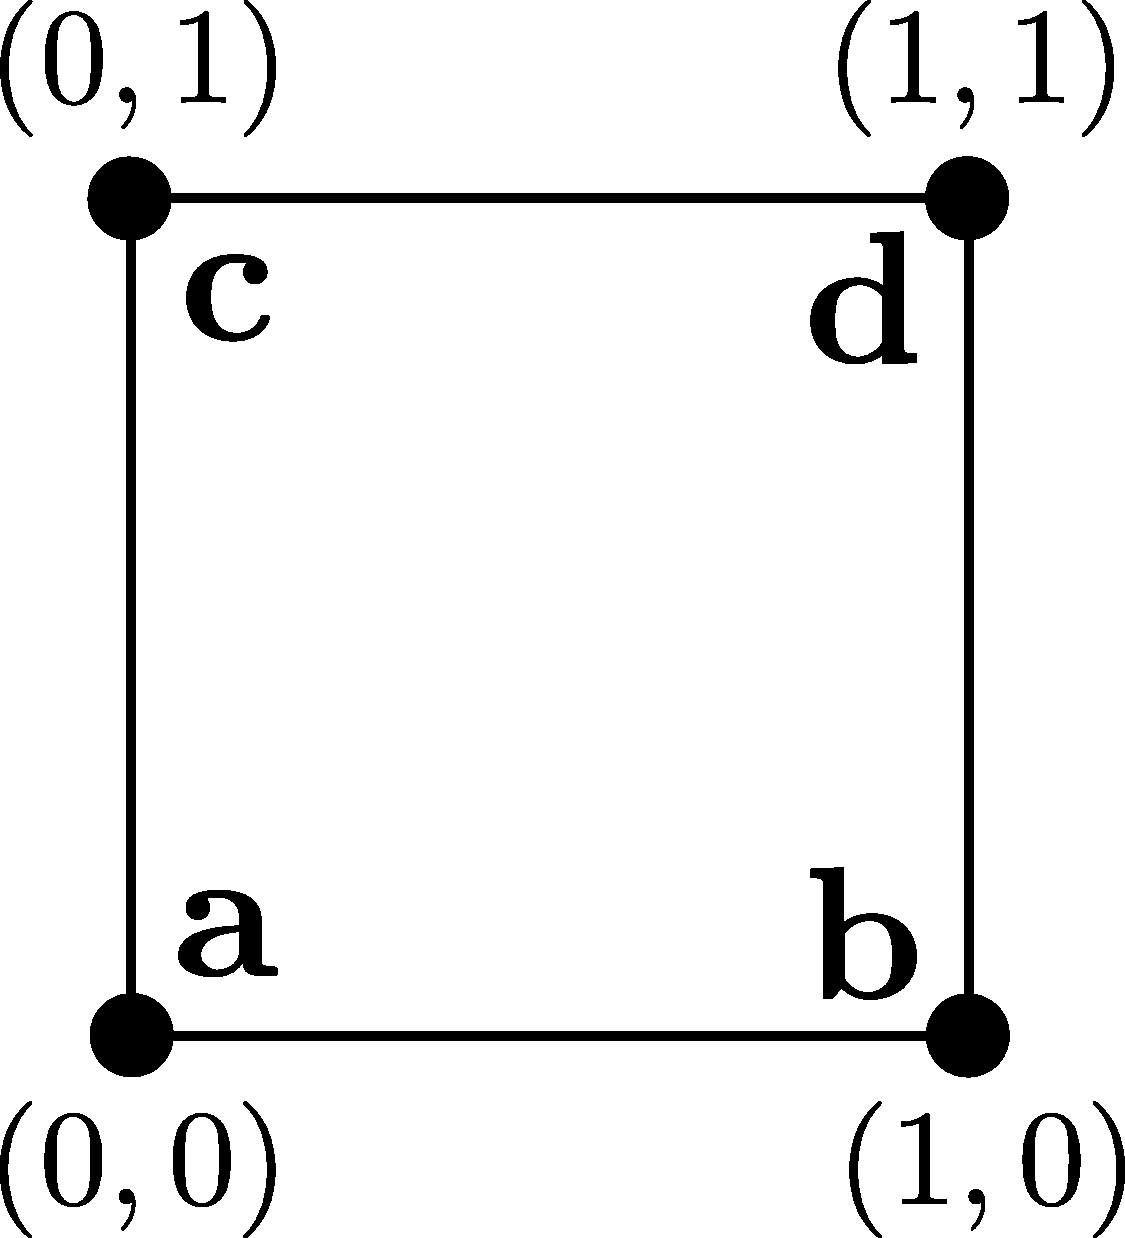
\includegraphics[width=1.5in]{figures/proportions_in_B2.pdf}
  \caption{The $36$ proportions in $\mathbb{B}^2$.}
\label{FIG:proportions_in_B2}
\end{figure}

All in all, this makes up to $36 = 8 + 6 \times 4 + 4$ proportions: $8$
proportions from the parallelogram $\mathbf{a}\mathbf{b}\mathbf{c}\mathbf{d}$,
$6 \times 4$ proportions from pairs of vertices, and $4$ proportions from the
$4$ vertices. This number of $36$ proportions could have been derived directly
by remembering that in $\mathbb{B}^2$ the proportions are defined in a
component-wise fashion, and that there are exactly $6$ valid patterns of
proportions in $\mathbb{B}$: as a proportion in $\mathbb{B}^2$ is the
concatenation of two proportions in $\mathbb{B}$, the number of valid
proportions in $\mathbb{B}^2$ necessarily is $6 \times 6 = 36$.

Note though that only $1 + 6 + 4 = 11$ of them can be considered
\textit{unique} (up to equivalence) and only one is non-flat. In section
\ref{SEC:number_of_parallelograms_in_Bm}, we will further investigate the
number of unique proportions that can be built in $\mathbb{B}^m$.

Going a dimension further can still be insightful. Figure \ref{FIG:cubes_in_B3}
illustrates the 12 non-flat proportions that exist in $\mathbb{B}^3$. These
proportions are the parallelograms making up the 6 faces of the left $3$-cube,
and six other \textit{diagonal} parallelograms on the $3$ remaining $3$-cubes.
The flat proportions are not shown for the sake of clarity.

\begin{figure}[!h]
\centering
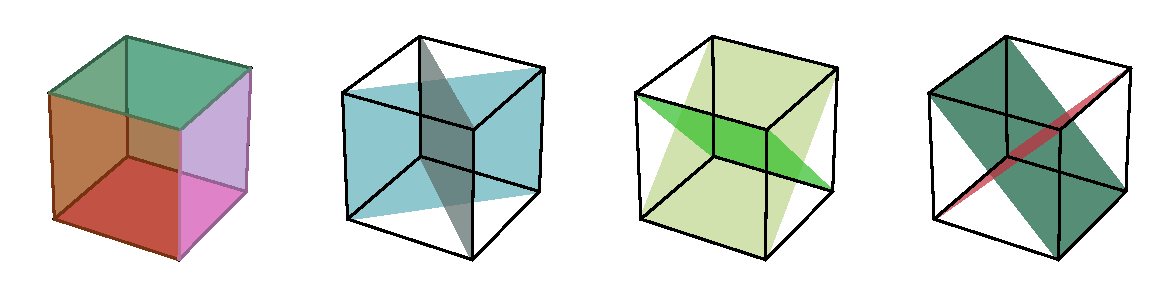
\includegraphics[width=\linewidth]{figures/cubes_in_B3.pdf}
  \caption{The twelve \textit{non-flat} parallelograms in $\mathbb{B}^3$: the
  six faces of the cube, and $3 \times 2$ \textit{diagonal} parallelograms,
  e.g. $(000) : (010) :: (101) : (111)$.}
\label{FIG:cubes_in_B3}
\end{figure}

Let us finally note the following remarkable property, which will be useful to
us much later in Chapter \ref{CHAP:analogy_preserving_functions}:

\begin{property}
  \label{PROPER:hamming_distance_boolean_proportion}
  Let $\mathbf{a}, \mathbf{b},\mathbf{c}, \mathbf{d}$ in $\mathbb{B}^m$, and
  let $H(\mathbf{x}, \mathbf{x'})$ be the Hamming distance between $\mathbf{x}$
  and $\mathbf{x'}$, i.e. the number of components we need to flip to transform
  $\mathbf{x}$ into $\mathbf{x'}$ (or the reverse).\\
  If $\mathbf{a} : \mathbf{b}
  :: \mathbf{c} : \mathbf{d}$, then these three equalities hold:

  $$
  \begin{cases}
    H(\mathbf{a}, \mathbf{b}) = H(\mathbf{c}, \mathbf{d})\\
    H(\mathbf{a}, \mathbf{c}) = H(\mathbf{b}, \mathbf{d})\\
    H(\mathbf{a}, \mathbf{d}) = H(\mathbf{b}, \mathbf{c}).
  \end{cases}
  $$
\end{property}

We can easily verify this property in $\mathbb{B}$ from Table
\ref{TAB:six_valid_patterns}, and the general case in $\mathbb{B}^m$ immediately
follows from Definition \ref{DEF:analogy_for_vectors}. Sadly, Property
\ref{PROPER:hamming_distance_boolean_proportion} only offers a necessary
condition for a proportion to hold, and not a sufficient one: indeed taking $a
= d = 1$ and $b = c =0$ in $\mathbb{B}$, the three equalities are clearly
respected but $1:0::0:1$ is not a valid proportion. We note that
while the first two properties $H(\mathbf{a}, \mathbf{b}) = H(\mathbf{c},
\mathbf{d})$ and $H(\mathbf{a}, \mathbf{c}) = H(\mathbf{b}, \mathbf{d})$ are
classical properties for parallelograms, the third one $H(\mathbf{a},
\mathbf{d}) = H(\mathbf{b}, \mathbf{c})$ is only true for rectangles. In fact,
the parallelograms that we can build in $\mathbb{B}^m$ are \textbf{always}
rectangles.

In this first section, starting from the three axioms of a general analogical
relation, we have given a first glimpse of Boolean proportions and their links
to the numerical arithmetic proportions. We also introduced the well-known
geometric proportion, but this one will not be considered in the rest of this
document. We also defined analogical proportions for vectors of Boolean or real
numbers, and we have seen that both the arithmetic and Boolean proportions
could be interpreted as relations between the four vertices of a parallelogram.
In the next section, we will apply our fresh knowledge to a classification
problem.

\section{Machine learning with Boolean proportions: a quick walk-through}
\label{SEC:machine_learning_with_boolean_proportions}

\paragraph{Problem setting\\}

We now have enough background on Boolean proportions to start doing some
machine learning. Here is our problem. We consider the set $\mathbb{B}^m$ and
its $2^m$ elements. For various $\mathbf{x} \in \mathbb{B}^m$, we know the
value of $f(\mathbf{x})$, where $f$ is a function from $\mathbb{B}^m$ to
$\mathbb{B}$.  The value $f(\mathbf{x})$ is called the \textbf{class} of
$\mathbf{x}$, or its \textbf{label}. The set $S \subsetneq \mathbb{B}^m$ of
elements for which $f(\mathbf{x})$ is known is called the \textbf{training
set}. For any element $\mathbf{x} \notin S$, $f(\mathbf{x})$ is unknown and our
goal is to guess it: this is a binary \textbf{classification problem}.

Suppose we're in $\mathbb{B}^3$ and consider Figure
\ref{FIG:classification_problem}.
\begin{figure}[!h]
\centering
  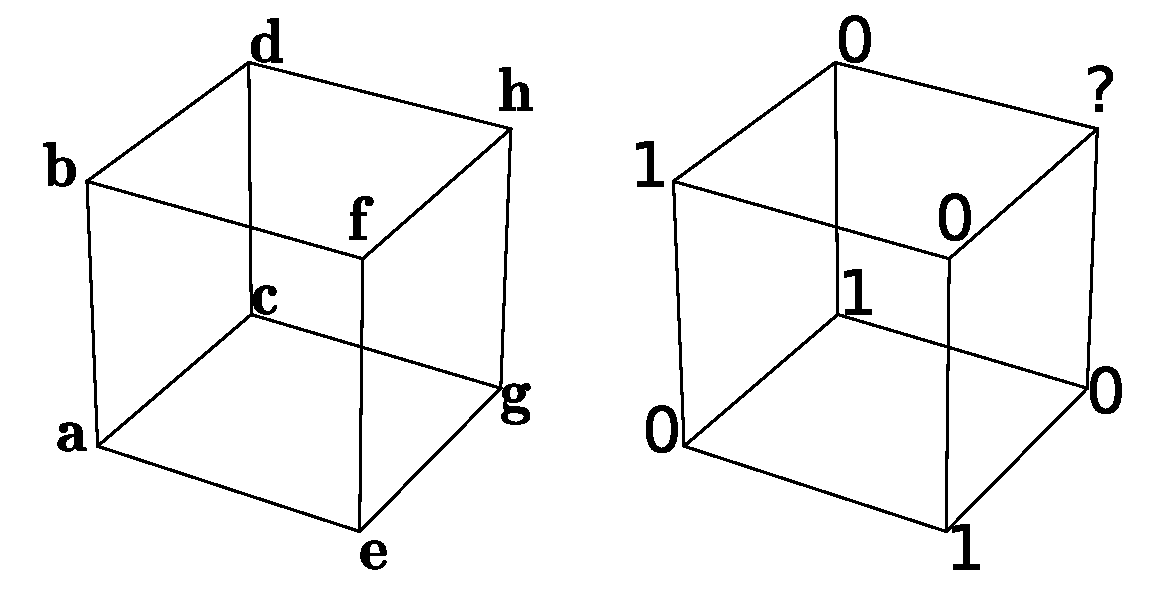
\includegraphics[width=3in]{figures/classification_problem.pdf}
  \caption{A classification problem in $\mathbb{B}^3$. Labels $f(\mathbf{x})$
  are on the right cube.}
\label{FIG:classification_problem}
\end{figure}
We know the values of $f(\mathbf{x})$ for
every single element $\mathbf{x}$ but $\mathbf{h}$, so $S = \{ \mathbf{a}, \mathbf{b},
\mathbf{c}, \mathbf{d}, \mathbf{e}, \mathbf{f}, \mathbf{g}\}$. There are
numerous methods at hand to go guess the value of $f(\mathbf{h})$. One of the
most famous one is the nearest neighbors heuristic, which would lead us to
consider that the label of $\mathbf{h}$ is the same as  that of its
\textit{neighbors}, i.e. the elements that are close to $\mathbf{h}$ with
respect to a given distance function. Using the Hamming distance, we would
assign to $\mathbf{h}$ the label $0$, because the $3$ closest neighbors of
$\mathbf{h}$, namely $\mathbf{d}, \mathbf{f}, \mathbf{g}$ all are labeled with
$0$.

\paragraph{The analogical inference principle\\}

Our point is here to describe the process of analogical classification, so we
will forget the nearest neighbor heuristic and we will instead make use of the
so-called \textbf{analogical inference principle}, which states that if four
elements $\mathbf{x}, \mathbf{y}, \mathbf{z}, \mathbf{t}$ are in proportion,
then their labels should also be in proportion:
$$
\infer[\text{Analogical inference principle}]{\mathbf{x} : \mathbf{y} ::
\mathbf{z} : \mathbf{t}}{f(\mathbf{x}) : f(\mathbf{y}) :: f(\mathbf{z}) :
f(\mathbf{t})}
$$

This is obviously an unsound principle, in that the conclusion does not
logically follows from the premise. But as we will see in this document, it can
still be useful.

The key point here is that if the value of $f(\mathbf{t})$ is unknown, it can
be \textbf{recovered} from the values of $f(\mathbf{x}), f(\mathbf{y}),
f(\mathbf{z})$ by the process of analogical equation solving that we explain
now.

\paragraph{Analogical equation solving\\}

We here want to guess the
value of $f(\mathbf{h})$. The analogical inference principle leads us to look
for all 3-tuples $(\mathbf{x}, \mathbf{y}, \mathbf{z}) \in S^3$ such that
$\mathbf{x}:\mathbf{y}::\mathbf{z}:\mathbf{h}$.  The principle then states that
for all of these $3$-tuples, we should have
$f(\mathbf{x}):f(\mathbf{y})::f(\mathbf{z}):f(\mathbf{h})$.
Figure \ref{FIG:cubes_in_B3} tells us that there are 6 (non-flat)
parallelograms involving $\mathbf{h}$ as a vertex. The six unique corresponding
proportions are:

\begin{enumerate}
  \item $\mathbf{a} : \mathbf{b} :: \mathbf{g} : \mathbf{h}$
  \item $\mathbf{a} : \mathbf{d} :: \mathbf{e} : \mathbf{h}$
  \item $\mathbf{a} : \mathbf{c} :: \mathbf{f} : \mathbf{h}$
  \item $\mathbf{b} : \mathbf{d} :: \mathbf{f} : \mathbf{h}$
  \item $\mathbf{e} : \mathbf{f} :: \mathbf{g} : \mathbf{h}$
  \item $\mathbf{c} : \mathbf{g} :: \mathbf{d} : \mathbf{h}$
\end{enumerate}

Applying the analogical inference principle to the first proportion $\mathbf{a}
: \mathbf{b} :: \mathbf{g} : \mathbf{h}$ leads to $f(\mathbf{a}) :
f(\mathbf{b}) :: f(\mathbf{g}) : f(\mathbf{h})$, which is equivalent to:
$$0:1::0:f(\mathbf{h}).$$ By referring to Table \ref{TAB:six_valid_patterns}, we
notice that $f(\mathbf{h})$ should be equal to $1$ for the proportion
$f(\mathbf{a}) : f(\mathbf{b}) :: f(\mathbf{g}) : f(\mathbf{h})$ to be a valid
one, because $0:1::0:1$. So we keep $1$ in the back of our head as a possible
candidate for $f(\mathbf{h})$: we say that $1$ is a \textbf{candidate
solution} for $f(\mathbf{h})$.

What we have just done is the \textbf{solving of an analogical equation}.
Generally speaking, an analogical equation is a proportion $a:b::c:x$ in a
context where $x$ is unknown. Determining the value of $x$ is then called the
\textit{solving} of this equation. Depending on the nature and values of $a, b$,
and $c$, there may or may not exist a solution, and it might not be unique. In a
Boolean setting, an equation is solvable for 6 patterns of $a, b, c$ (the 6
patterns of Table \ref{TAB:six_valid_patterns}, naturally). As we can see, the
solution is always unique:

\begin{proposition}
  \label{PROPOS:equation_solving}
  Let $a, b, c$ in $\mathbb{B}$. The analogical equation
  $a :b::c:x$
  is solvable if and only if $a = b$ or $a = c$. The solution denoted
  $\emph{sol}(a, b, c)$ is then given by:
  $$
  \begin{cases}
    \emph{sol}(a, b, c) \eqdef c \emph{ if } a = b,\\
    \emph{sol}(a, b, c) \eqdef b \emph{ if } a = c,
  \end{cases}
  $$
  or more generally:
  $$\emph{sol}(a, b, c) \eqdef c - a + b,$$
  because the Boolean proportion is a particular case of the arithmetic
  proportion.
\end{proposition}

Let's get back to the estimation of $f(\mathbf{h})$. Applying the analogical
inference principle to the second proportion $\mathbf{a} : \mathbf{d} ::
\mathbf{e} : \mathbf{h}$ leads $f(\mathbf{a)} : f(\mathbf{d}) :: f(\mathbf{e})
: f(\mathbf{h})$, and to the solving of $0:0::1:f(\mathbf{h})$. Here again, the
solution is $1$, just like the candidate of the first proportion.
The third proportion  $\mathbf{a} : \mathbf{c} :: \mathbf{f} : \mathbf{h}$
leads to the solving of $0:1::0:f(\mathbf{h})$, also claiming that $1$ is a good candidate.

And now the fourth proportion $\mathbf{b} : \mathbf{d} :: \mathbf{f} :
\mathbf{h}$, which leads to $1:0::0:f(\mathbf{h})$. \textbf{This equation is not
solvable}: neither $1:0::0:1$ nor $1:0::0:0$ are valid proportions. We thus
simply discard the proportion $\mathbf{b} : \mathbf{d} :: \mathbf{f} :
\mathbf{h}$ as a potential source of information about $f(\mathbf{h)}$, because
we are not in a position to apply the analogical inference principle. We can
easily verify that the fifth and sixth proportions also lead to non-solvable
equations.

\paragraph{Estimation of $f(\mathbf{h})$\\}

All in all, we are left with three candidates coming from the first three
proportions, all of which are equal to $1$. Our guess will thus be that
$f(\mathbf{h})$ should be equal to $1$, so we will set the \textbf{estimation} of
$f(\mathbf{h}$ as $\hat{f}(\mathbf{h}) = 1$. Is this correct? Well in real-world
settings, there is no way to know for sure, because the ground truth function
$f$ is unknown (otherwise, there is no point in trying to classify $\mathbf{h}$
in the first place).

Notice that we have so far lightheartedly ignored  all the flat proportions,
i.e. proportions where the four elements are not all distinct.
This is because none of these proportions allow us to derive a solvable
equation. Considering for example $\mathbf{d} : \mathbf{h} :: \mathbf{d} :
\mathbf{h}$, we're led to the solving of $f(\mathbf{d}) : f(\mathbf{h}) ::
f(\mathbf{d}) : f(\mathbf{h})$, or equivalently of $0 : f(\mathbf{h}) :: 0 :
f(\mathbf{h})$. Both values $0$ and $1$ could lead to equally valid proportions
here, so there is simply no predictive power in the flat proportions. We have
also only considered unique proportions, up to equivalence. The first proportion
$\mathbf{a} : \mathbf{b} :: \mathbf{g} : \mathbf{h}$ for example is equivalent
to $\mathbf{a} : \mathbf{g} :: \mathbf{b} : \mathbf{h}$ (using central
permutation), which we could have
used instead. As any two equivalent proportions lead to the same solution for
their associated class equations, we usually choose to ignore all other equivalent
proportions, which allows to divide the number of equation solving by a factor
of $2$.

\paragraph{The analogical classification process: summary\\}

Here is a small outline of our classification process, that was entirely
governed by the analogical inference principle. Our goal was to guess the value
of $f(\mathbf{h})$:

\begin{itemize}
  \item We first looked at all the $(\mathbf{x}, \mathbf{y}, \mathbf{z}) \in
    \mathbf{B}^3$ such that:
    \begin{itemize}
      \item $f(\mathbf{x}), f(\mathbf{y})$ and $f(\mathbf{z})$ are known ;
      \item $\mathbf{x}:\mathbf{y}::\mathbf{z}:\mathbf{h}$ holds ;
      \item the \textbf{class equation} $f(\mathbf{x}) :f(\mathbf{y}) ::
        f(\mathbf{z}) :s$ is \textbf{solvable}. $s$ is called a
        \textbf{candidate solution}.
    \end{itemize}
    Each of our three candidate solutions $s_1, s_2, s_3$ agreed on the same prediction:
    $s_i = 1$ for all $i$.
  \item We thus estimated that $f(\mathbf{h})$ should indeed be equal to $1$.
\end{itemize}

This minimal example of analogical classification raises a few concerns, which
we will be thoroughly addressed in this document:
\begin{enumerate}
  \item All of the three candidate solutions for $f(\mathbf{h})$ agreed on the
    same prediction: $1$. What if one of them predicted $0$? A first drastic
    option is to refuse to classify $\mathbf{h}$, on the basis that if the
    candidates cannot agree on their predictions, then we should not trust any
    of them. As it will become clear, in practice the candidates never really
    completely agree, even though sometimes a clear majority emerges. So this
    strategy would make the prediction impossible for most elements $\mathbf{x}
    \notin S$. A wiser option is to consider an aggregation of the candidate
    solutions: the most common one, for example. This is the option that has
    been took on so far, as we will see in the next chapter.
  \item Here, by chance, the set of candidate solutions for $f(\mathbf{h})$ was
    not empty: we found three candidate solutions. What happens if we can't
    find any candidate? This case arises when there are no 3-tuple
    $(\mathbf{x}, \mathbf{y}, \mathbf{z}) \in S^3$ such that $\mathbf{x} :
    \mathbf{y}::\mathbf{z}:\mathbf{h}$ and such that the associated equation
    $f(\mathbf{x}):f(\mathbf{y})::f(\mathbf{z}):f(\mathbf{h})$ is solvable. In
    the works of Stroppa and Yvon (\cite{StrYvoCNLL05}), such an $\mathbf{h}$
    cannot be classified. The notion of \textbf{analogical dissimilarity} as
    used in \cite{BayMicDelIJCAI07} will allow to bypass this issue. In the
    next chapter, we will detail these two version of analogical learning, and
    one of the contribution of our work is to provide a unifying view of the
    two techniques.
  \item How \textit{safe} is the analogical inference principle? What are some
    theoretical guarantees that could allow us to use it on a sound basis? This
    question stays, to this day, unanswered. In Chapter \ref{TODO} however, we
    will provide a complete characterization of the Boolean functions $f$ that
    allow to derive sound conclusions.
\end{enumerate}

Before moving further to the next section, let us  consider a seemingly trivial
question: how many proportions can we build in $\mathbb{B}^m$? As we will see,
this question will provide us some further insight about Boolean proportions.
This last discussion is, however, not as important as the previous ones and can
safely be ignored by the impatient reader.

\paragraph{How many proportions can we build in $\mathbb{B}^m$?\\}
\label{SEC:number_of_parallelograms_in_Bm}

Exactly $6^m$! And it is fairly easy to derive: there are $6$ proportions in
$\mathbb{B}$. As a proportion in $\mathbb{B}^2$ is the concatenation of any two
proportions in $\mathbb{B}$, there are exactly $6^2 = 36$ proportions in
$\mathbb{B}^2$, as seen in Section
\ref{SEC:shortcut_from_aristotle_to_boolean_proportions}. Analogical
proportions in $\mathbb{B}^m$ are defined component-wise, i.e. they are the
concatenation of $m$ proportions in $\mathbb{B}$. Equivalently, a proportion in
$\mathbb{B}^m$ is the concatenation of a proportion in $\mathbb{B}^{m - 1}$ and
a proportion in $\mathbb{B}$. By trivial induction, we can build $6^m$
proportions in $\mathbb{B}^m$.

But let's now ask a more relevant and challenging question: \textbf{how many
\textit{useful} proportions can we build in $\mathbb{B}^m$?} By
\textit{useful}, we mean proportions that could be used for classification
purposes.  We have seen in Section \ref{TODO} that the only proportions
$\mathbf{a} : \mathbf{b} :: \mathbf{c} : \mathbf{d}$ that are useful for
classification purposes are those where all elements $\mathbf{a}, \mathbf{b},
\mathbf{c}, \mathbf{d}$ are distinct, i.e. the non-flat proportions. We thus
want to exclude from the $6^m$ proportions those that comply with one of the
following patterns:

\begin{itemize}
  \item $\mathbf{a}: \mathbf{a} :: \mathbf{a} : \mathbf{a}$
  \item $\mathbf{a}: \mathbf{b} :: \mathbf{a} : \mathbf{b}$, and its three
    equivalent forms $\mathbf{a}: \mathbf{a} :: \mathbf{b} : \mathbf{b}$,~
    $\mathbf{b}: \mathbf{a} :: \mathbf{b} : \mathbf{a}$, and $\mathbf{b}:
    \mathbf{b} :: \mathbf{a} : \mathbf{a}$
\end{itemize}

Now, let's count them.

\begin{itemize}
  \item Each of the $2^m$ vertex $\mathbf{a}$ will generate a proportion of the
    form $\mathbf{a}: \mathbf{a} :: \mathbf{a} : \mathbf{a}$, so there are
    exactly $2^m$ proportions of this kind.
  \item Every pair $(\mathbf{a}, \mathbf{b})$ of vertices will generate four
    proportions:
    \begin{itemize}
      \item $\mathbf{a}: \mathbf{b} :: \mathbf{a} : \mathbf{b}$,
      \item $\mathbf{a}: \mathbf{a} :: \mathbf{b} : \mathbf{b}$,
      \item $\mathbf{b}: \mathbf{a} :: \mathbf{b} : \mathbf{a}$,
      \item $\mathbf{b}: \mathbf{b} :: \mathbf{a} : \mathbf{a}$.
    \end{itemize}
    There are $\binom{2^m}{2}$ distinct pairs of vertices, so in total this
    makes $4\cdot \binom{2^m}{2}$ proportions of the form $\mathbf{a}: \mathbf{b} ::
    \mathbf{a} : \mathbf{b}$ with its equivalent forms.
\end{itemize}

We are then left with the number of $6^m - 2^m - 4\cdot\binom{2^m}{2}$ useful
proportions. We know that for each of these proportions, all elements
$\mathbf{a}, \mathbf{b}, \mathbf{c}, \mathbf{d}$  are distinct. For each of
them, there are thus 7 other equivalent forms, which reduces the number of
useful and unique (up to equivalence) proportions to:
$$P_m = \frac{1}{8} \left[6^m - 2^m - 4\cdot\binom{2^m}{2} \right].$$
Table \ref{TAB:n_params_in_cube} gives the values of $P_m$ for the first $10$
values of $m$.
\begin{table}[h!]
\centering
  \begin{tabular}{ l  l }
\toprule
 $m$ & $P_m$\\
\midrule
    1	&	0\\
    2 &	1\\
    3	&	12\\
    4	&	100\\
    5 &	720\\
    6 &	4816\\
    7 &	30912\\
    8 &	193600\\
    9 & 1194240\\
    10 & 7296256\\
\bottomrule
\end{tabular}
\caption{Number of unique non-flat proportions in an $m$-dimensional cube.}
\label{TAB:n_params_in_cube}
\end{table}
Naturally, $P_2$ and $P_3$ are in accordance with our empirical  results from
Figures \ref{FIG:proportions_in_B2} and \ref{FIG:cubes_in_B3}. The fact that
$P_1 = 0$ means that no inference can be done with analogical proportion in
$\mathbb{B}$, which is perfectly normal: in $\mathbb{B}$, all proportions are
flat (i.e. the pattern is always $a:b::a:b$ or $a:a::b:b$).

In fact, it turns out that this sequence of numbers $0, 1, 12, 100\dots$ is
already known as the sequence named A016283 from the OEIS\footnote{The On-line
Encyclopedia of Integer Sequences (http://oeis.org/A016283)}.
This sequence actually describes \textit{the number of rectangles that can be
formed from the vertices of an $m$-dimensional cube}, which is exactly
equivalent to the number of \textit{useful} proportions that we wanted to
compute. The formula given by the OEIS is:
$$P_m = \frac{6^m}{8} - 4^{m - 1} + 2^{m - 3},$$
and using the fact that $\binom{n}{k} = \frac{n}{k}\binom{n - 1}{k - 1}$, it
can be shown that the two formulas $\frac{1}{8} \left[6^m - 2^m -
4\cdot\binom{2^m}{2} \right]$ and $\frac{6^m}{8} - 4^{m - 1} + 2^{m- 3}$ are,
fortunately, equivalent.  To be fair, we have no idea how the formula of the
OEIS was derived, but we firmly believe that ours is the most entertaining one!

This closes our informal introduction to analogical classification and
analogical proportions. The next section will be devoted to more formal
definition of analogical proportion in different settings, and analogical
classification will be more detailed in Chapter
\ref{CHAP:functional_definition}.

\section{Formal definitions}
\label{SEC:formal_definitions_proportions}

The Boolean proportion was introduced in the previous section in an informal
way, along with many key concepts such as the solving on an analogical
equation, and the analogical inference principle. In this section, we will
provide the definition of the Boolean proportion (and others) in a more formal
way.

\paragraph{A factorization-based definition of analogical proportions\\}

Probably the first use of formal proportions is that of Lepage in \cite{Lep04}
who, starting from the three aforementioned axioms, formally defined analogical
proportions over alphabets of letters with the aim of generating (analogical)
formal languages. His definition have later been generalized in the works of
Stroppa and Yvon (see \cite{StrYvoCNLL05} and \cite{StrYvoREPORT05}), who
provided an algebraic factorization-based definition of analogical proportions
in semigroups:

\begin{definition}
\label{DEF:proportion_semi_group}
Let $(U, \oplus)$ be a semigroup, i.e. $U$ is a set and $\oplus$ is an
  associative binary operation. Four elements $a, b, c, d \in U$, are in proportion if
  there exist some factorization
  \begin{align*}
    a &= a_1 \oplus a_2 \oplus \cdots \oplus a_n\\
    b &= b_1 \oplus b_2 \oplus \cdots \oplus b_n\\
    c &= c_1 \oplus c_2 \oplus \cdots \oplus c_n\\
    d &= d_1 \oplus d_2 \oplus \cdots \oplus d_n,
  \end{align*}

  such that for all $i \in [1, n]$, 
  $$
  \begin{cases}
    a_i = b_i \text{ and } c_i = d_i\\
    \text{or}\\
    a_i = c_i \text{ and } b_i = d_i.
  \end{cases}
  $$
\end{definition}

\noindent
We can clearly foresee here the features of the Boolean proportion.

\begin{testexample}
It will be
insightful to instantiate $U$ as the set of natural number $\mathbb{N}$ and
$\oplus$ as the usual multiplication $\times$. In this setting, let's consider
the prime factorization of:

\begin{align*}
  a &= 30 = 1 \times 2 \times 3 \times 5\\
  b &= 60 = 2 \times 2 \times 3 \times 5\\
  c &= 25 = 1 \times 1 \times 5 \times 5\\
  d &= 50 = 2 \times 1 \times 5 \times 5
\end{align*}

For each $i$, we either have $a_i = b_i$ and $c_i = d_i$ ($i = 2, 3, 4$) or
$a_i = c_i$ and $b_i = d_i$ ($i = 1, 4$). We can then say that $a, b, c, d$ are
in proportion, i.e. $30: 60 :: 25:50$. Naturally, the reader will recognize
here the geometric proportion: $\frac{30}{60} = \frac{25}{50}$.
\end{testexample}

\begin{testexample}
  Another use of this Definition can be found in \cite{StrYvoREPORT05}, where
  the authors define an analogy between words of a finite alphabet using the
  concatenation operator, which allows to build proportions such as:
  $$\text{eat} : \text{eating} :: \text{look} : \text{looking}.$$ This analogy
  was used in an automatic verb conjugation task that will be briefly descibed
  in Section \ref{SEC:conservative_classifier}.
\end{testexample}


Starting from the general lines of Definition \ref{DEF:proportion_semi_group},
other proportions have been defined in various domains, namely analogies
between trees, lattices, or matrices \cite{MicDel04, StrYvoREPORT05,
MicBayDelJAIR08}. However, we will not detail them further here and rather
focus on other domains of interest.

\paragraph{Analogical proportions between sets\\}

In \cite{Lep03}, Lepage defines an analogy between sets as follows: four subsets
$A, B, C, D$ of a universal set $X$ are in proportion if $A$ can be transformed
into $B$ by adding and deleting the same elements as to transform $C$ into $D$.
A more formal definition has been given in \cite{StrYvoREPORT05}:

\begin{definition}
  \label{DEF:analogy_set_facto}
  Let $A, B, C, D \subset X$. $A, B, C, D$ are in proportion if there exists
  four subsets $U, V, W$ and $Z$ (not necessarily disjoint) such that:
  $$
  \begin{cases}
    A = U \cup V\\
    B = U \cup W\\
    C = Z \cup V\\
    D = Z \cup W\\
  \end{cases}
  $$
\end{definition}

To go from $A$ to $B$, one needs to add $W$ and remove $V$. To go from $C$ to
$D$, one needs to do the exact same thing: add $W$ and remove $V$. An
equivalent definition has been given in \cite{MicPra09}:

\begin{definition}
  \label{DEF:analogy_set_miclet_henri}
  Let $A, B, C, D \subset X$. $A, B, C, D$ are in proportion if:
  $$
  A \setminus B = C \setminus D \text{ and } B \setminus A = D \setminus A
  $$
\end{definition}

Definition \ref{DEF:analogy_set_miclet_henri} reads as \textit{$A$ differs from
$B$ as $C$ differs from $D$, and $B$ differs from $A$ as $D$ differs from $C$},
which is naturally equivalent to the statement of Definition
\ref{DEF:analogy_set_facto}: $A \setminus B = C \setminus D = V$, and $B
\setminus A = D \setminus A  = W$.  Finally, a last equivalent definition can
be given as follows (not without using various ingenious tweaks):

\begin{definition}
  \label{DEF:yet_other_equiv_def}
  Let $A, B, C, D \subset X$. $A, B, C, D$ are in proportion if:
  $$A \cup D = B \cup C \text{ and } A \cap D = B \cap C.$$
\end{definition}

\noindent
These three equivalent definitions are illustrated in Figure
\ref{FIG:equiv_analogies_sets}.

\begin{figure}[!h]
\centering
  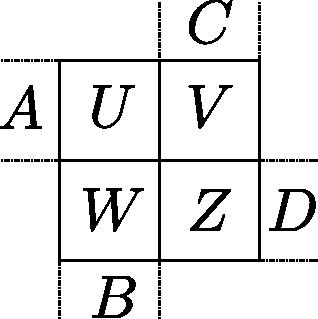
\includegraphics[width=1in]{figures/subset_analogies.pdf}
  \caption{The four sets $A, B, C, D$ are in proportion.}
\label{FIG:equiv_analogies_sets}
\end{figure}

\begin{testexample}
For a more concrete example, let us consider $A = \{a, b, c, g\}, B = \{a, b,
d, e, g\}, C = \{c, f, g\}$ and $D = \{d, e, f, g\}$, as summed-up in Table
\ref{TAB:analogy_sets}.
Setting $U = \{a, b, g\}, V = \{c\}, W = \{d, e\}$ and $Z = \{f, g\}$, the
conditions of Definition  \ref{DEF:analogy_set_facto}  are clearly satisfied.
Also, $A \setminus B = C \setminus D = \{c\} = V$, and $B\setminus A = D
\setminus C = \{d, e\} = W$. Finally, $A \cup D = B \cup C = \{a, b, c, d, e,
f, g\}$ and $A\cap D = B\cap C = \{g\}$.
\end{testexample}
\begin{table}[h!]
\centering
$$
\begin{tabular}{ c  c  c  c  c  c  c  c }
\toprule
  & a & b & c & d & e & f & g\\
\midrule
  A & \times & \times & \times &  &  &  & \times \\
  B & \times & \times &  & \times & \times &  & \times\\
  C &  &  & \times &  &  & \times & \times\\
  D &  &  &  & \times & \times & \times & \times\\
\bottomrule
\end{tabular}
$$
\caption{Four sets $A, B, C, D$ in analogical proportion.}
\label{TAB:analogy_sets}
\end{table}

\paragraph{Formal definition of the Boolean proportion\\}

We are now in a position to give a formal definition of the Boolean proportion,
which can be directly derived from Definition
\ref{DEF:analogy_set_miclet_henri} by considering the set $\mathbb{B} = \{0,
1\}$:

\begin{definition}
  \label{DEF:boolean_proportion}
  Four elements $a, b, c, d$ in $\mathbb{B} = \{0, 1\}$ are in proportion if
  \begin{alignat*}{2}
    &(a \leftrightarrow b \wedge c \leftrightarrow d) && \vee (a
    \leftrightarrow c \wedge b \leftrightarrow d), \text{ or equivalently}\\
     & (a \wedge d \leftrightarrow b \wedge c) &&\wedge (a \vee  d
    \leftrightarrow b \vee c),
  \end{alignat*}
  where $\leftrightarrow$ stands for the equivalence connective. The second
  expression directly comes from Definition \ref{DEF:yet_other_equiv_def}
\end{definition}

These scary formulas state the exact same facts as the previous definitions,
i.e. that $a$ differs from $b$ as $c$ differs from $d$ and conversely $b$
differs from $a$ as $d$ differs from $c$. Naturally, Definition
\ref{DEF:boolean_proportion} and \ref{DEF:boolean_proportion_informal} (the one
we initially suggested) are equivalent.

\paragraph{Pioneering works: Klein and Piaget\\}

We cannot talk about formal Boolean proportions without going back to the 80's
and mention the pioneering work of Sheldon Klein who, to some extent, defined
his \textit{own} Boolean analogical proportion \cite{Kle83}. His definition
states that $a, b, c, d$ in $\mathbb{B}$ are in proportion if $a \oplus b = c
\oplus d$, where $\oplus$ is the XOR operator.  This definition is less
restrictive than Definition \ref{DEF:boolean_proportion}, and amounts to
considering that in addition to the $6$ valid patterns from Table
\ref{TAB:six_valid_patterns}, two other patterns are also valid, namely
$0:1::1:0$ and its counterpart $1:0::0:1$.

These two patterns seem appealing at first sight, because they capture the fact
that $a : \neg a :: b \neg b$. However, they also lead to the fact that
$a:b::c:d \iff b : a :: c :d$, which seems quite unnatural for an analogy.
Indeed, the pattern $b:a::c:d$ is not in the same equivalent class as the
pattern $a:b::c:d$ as we have seen in Section
\ref{SEC:shortcut_from_aristotle_to_boolean_proportions}. In practice, it is
often observed that using the modeling of Klein leads to less accuracte
learners than using the standard modeling.

Another remarkable precursor work is that of Jean Piaget who, in the annex of a
French book from 1952 \cite{Pia52}, defined what he called a \textit{logical
proportion} as follows: four propositions $a, b, c,d$ are in proportion if $(a
\wedge d \leftrightarrow b \wedge c) \wedge (a \vee  d \leftrightarrow b \vee
c)$. This definition is clearly equivalent to what we refer to now as the
Boolean proportion, but the fact is that Piaget never made any reference to
analogy in this work.

The notion of Boolean analogical proportion has recently been extended to the
concept of \textbf{logical proportion} (see e.g. \cite{PraRic14}), but their
details are out of the scope of this document.

\section*{Conclusion}
